%!TEX program = xelatex
%# -*- coding: utf-8 -*-
%!TEX encoding = UTF-8 Unicode

\documentclass[12pt,oneside,a4paper]{article}\usepackage[]{graphicx}\usepackage[]{xcolor}
%% maxwidth is the original width if it is less than linewidth
%% otherwise use linewidth (to make sure the graphics do not exceed the margin)
\makeatletter
\def\maxwidth{ %
  \ifdim\Gin@nat@width>\linewidth
    \linewidth
  \else
    \Gin@nat@width
  \fi
}
\makeatother

\definecolor{fgcolor}{rgb}{0, 0, 0}
\newcommand{\hlnum}[1]{\textcolor[rgb]{0,0,0}{#1}}%
\newcommand{\hlstr}[1]{\textcolor[rgb]{0,0,1}{#1}}%
\newcommand{\hlcom}[1]{\textcolor[rgb]{0.443,0.478,0.702}{#1}}%
\newcommand{\hlopt}[1]{\textcolor[rgb]{0,0,0}{#1}}%
\newcommand{\hlstd}[1]{\textcolor[rgb]{0,0,0}{#1}}%
\newcommand{\hlkwa}[1]{\textcolor[rgb]{0.498,0,0.333}{\textbf{#1}}}%
\newcommand{\hlkwb}[1]{\textcolor[rgb]{0.498,0,0.333}{\textbf{#1}}}%
\newcommand{\hlkwc}[1]{\textcolor[rgb]{0.498,0,0.333}{\textbf{#1}}}%
\newcommand{\hlkwd}[1]{\textcolor[rgb]{0,0,0}{#1}}%

\usepackage{framed}
\makeatletter
\newenvironment{kframe}{%
 \def\at@end@of@kframe{}%
 \ifinner\ifhmode%
  \def\at@end@of@kframe{\end{minipage}}%
  \begin{minipage}{\columnwidth}%
 \fi\fi%
 \def\FrameCommand##1{\hskip\@totalleftmargin \hskip-\fboxsep
 \colorbox{shadecolor}{##1}\hskip-\fboxsep
     % There is no \\@totalrightmargin, so:
     \hskip-\linewidth \hskip-\@totalleftmargin \hskip\columnwidth}%
 \MakeFramed {\advance\hsize-\width
   \@totalleftmargin\z@ \linewidth\hsize
   \@setminipage}}%
 {\par\unskip\endMakeFramed%
 \at@end@of@kframe}
\makeatother

\definecolor{shadecolor}{rgb}{.97, .97, .97}
\definecolor{messagecolor}{rgb}{0, 0, 0}
\definecolor{warningcolor}{rgb}{1, 0, 1}
\definecolor{errorcolor}{rgb}{1, 0, 0}
\newenvironment{knitrout}{}{} % an empty environment to be redefined in TeX

\usepackage{alltt}
\usepackage{geometry}
\geometry{verbose,tmargin=2cm,bmargin=2cm,lmargin=2cm,rmargin=2cm}
\usepackage[pdfusetitle,
 bookmarks=true,bookmarksnumbered=true,bookmarksopen=true,bookmarksopenlevel=2,
 breaklinks=false,pdfborder={0 0 1},backref=false,colorlinks=false]
 {hyperref}
\hypersetup{pdfstartview={XYZ null null 1}}
\usepackage{url}
\setcounter{secnumdepth}{2}
\setcounter{tocdepth}{2}
\usepackage{microtype}

\usepackage{amsmath, amsthm, amssymb, amsfonts}

\usepackage{algorithm}
\usepackage{algorithmic}
\renewcommand{\algorithmicrequire}{\textbf{Input:}} 
\renewcommand{\algorithmicensure}{\textbf{Output:}} 

\usepackage[sc]{mathpazo}
\linespread{1.1}
\usepackage[T1]{fontenc}


\usepackage{graphics}
\usepackage{graphicx}
\usepackage[figure]{hypcap}
\usepackage[hypcap]{caption}
\usepackage{tikz}
%\usepackage{grffile} 
%\usepackage{float} 
\usepackage{pdfpages}

\usepackage{multirow}
\usepackage{booktabs}
\usepackage{threeparttable}

%\usepackage[square,numbers,super,comma,sort]{natbib}
%\usepackage[backend=biber, style=nature, sorting=none, isbn=false, url=false, doi=false]{biblatex}
%\addbibresource{ref.bib}
%\usepackage[]{authblk}

\usepackage{verbatim}

\usepackage{fancyhdr}
\usepackage{extramarks}
\lhead{\hmwkAuthorName}
\chead{\hmwkClass\ (\hmwkClassInstructor\ \hmwkClassTime): \hmwkTitle}
\rhead{\firstxmark}
\lfoot{\lastxmark}
\cfoot{\thepage}

\newenvironment{problem}[2][Problem]{\begin{trivlist}
\item[\hskip \labelsep {\bfseries #1}\hskip \labelsep {\bfseries #2.}]}{\end{trivlist}}


\newcommand{\enterProblemHeader}[1]{
    \nobreak\extramarks{}{Problem \arabic{#1} continued on next page\ldots}\nobreak{}
    \nobreak\extramarks{Problem \arabic{#1} (continued)}{Problem \arabic{#1} continued on next page\ldots}\nobreak{}
}

\newcommand{\exitProblemHeader}[1]{
    \nobreak\extramarks{Problem \arabic{#1} (continued)}{Problem \arabic{#1} continued on next page\ldots}\nobreak{}
    \stepcounter{#1}
    \nobreak\extramarks{Problem \arabic{#1}}{}\nobreak{}
}


\setcounter{secnumdepth}{0}
\newcounter{partCounter}
\newcounter{homeworkProblemCounter}
\setcounter{homeworkProblemCounter}{1}
\nobreak\extramarks{Problem \arabic{homeworkProblemCounter}}{}\nobreak{}



\newenvironment{homeworkProblem}[1][-1]{
    \ifnum#1>0
        \setcounter{homeworkProblemCounter}{#1}
    \fi
    \section{Problem \arabic{homeworkProblemCounter}}
    \setcounter{partCounter}{1}
    \enterProblemHeader{homeworkProblemCounter}
}{
    \exitProblemHeader{homeworkProblemCounter}
}


\newcommand{\hmwkTitle}{Homework\ \#2}
\newcommand{\hmwkDueDate}{February 12, 2014}
\newcommand{\hmwkClass}{Calculus}
\newcommand{\hmwkClassTime}{Section A}
\newcommand{\hmwkClassInstructor}{Professor Isaac Newton}
\newcommand{\hmwkAuthorName}{Josh Davis}



\title{
    \vspace{2in}
    \textmd{\textbf{\hmwkClass:\ \hmwkTitle}}\\
    \normalsize\vspace{0.1in}\small{Due\ on\ \hmwkDueDate\ at 3:10pm}\\
    \vspace{0.1in}\large{\textit{\hmwkClassInstructor\ \hmwkClassTime}}
    \vspace{3in}
}


\author{\textbf{\hmwkAuthorName}}
\date{}

\renewcommand{\part}[1]{\textbf{\large Part \Alph{partCounter}}\stepcounter{partCounter}\\}



%\renewcommand{\qedsymbol}{\filledbox}
%Good resources for looking up how to do stuff:
%Binary operators: http://www.access2science.com/latex/Binary.html
%General help: http://en.wikibooks.org/wiki/LaTeX/Mathematics
%Or just google stuff
\IfFileExists{upquote.sty}{\usepackage{upquote}}{}
\begin{document}

\maketitle

\pagebreak
 


\begin{problem}{2.1}
Height and weight data (Data file: Htwt) The table below and the data file give ht = height in centimeters and wt = weight in kilograms for a sample of n  =  10 18-year-old girls. The data are taken from a larger study described in Problem 3.3. Interest is in predicting weight from height.

\begin{table}[ht!]
\centering
\caption{Problem 1}
\begin{tabular}{rr}
\toprule
 \multicolumn{1}{c}{ ht } & \multicolumn{1}{c}{ wt } \\
\midrule
 $169.6$ & $71.2$ \\
 $166.8$ & $58.2$ \\
 $157.1$ & $56$ \\
 $181.1$ & $64.5$ \\
 $158.4$ & $53$ \\
 $165.6$ & $52.4$ \\
 $166.7$ & $56.8$ \\
 $156.5$ & $49.2$ \\
 $168.1$ & $55.6$ \\
 $165.3$ & $77.8$ \\
\bottomrule
\end{tabular}
\label{Problem 1}
\end{table}

\end{problem} 

\begin{problem}{2.1.1} Draw a scatterplot of wt on the vertical axis versus ht on the horizontal axis. On the basis of this plot, does a simple linear regression model make sense for these data? Why or why not?
\end{problem}

\begin{knitrout}
\definecolor{shadecolor}{rgb}{1, 1, 1}\color{fgcolor}

{\centering 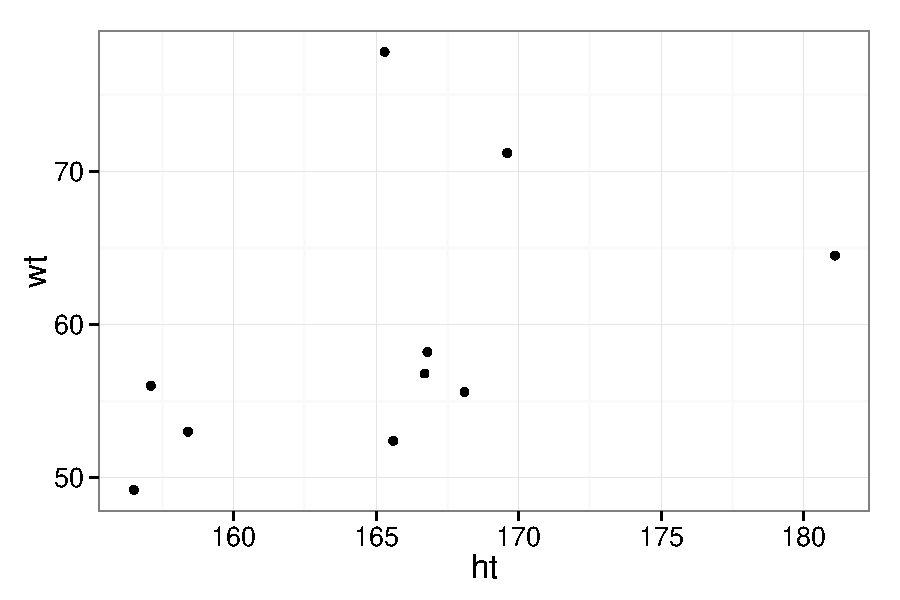
\includegraphics[width=.6\linewidth]{figure/p211} 

}



\end{knitrout}

Yes, except for some extreme outliers, the linear ascending tendency of wt over ht is obvious.

\begin{problem}{2.1.2} Show that $\bar{x} = 165.52$ , $\bar{y} = 59.47$ , $S_{XX}  =  472.08$, $S_{YY}  =  731.96$, and $S_{XY} = 274.79$. Compute estimates of the slope and the intercept for the regression of Y on X. Draw the fitted line on your scatterplot.
\end{problem}

$$\bar{x} = \frac{\sum_{i = 1}^{10}{x_{i}}}{n} = 165.52$$
$$\bar{y} = \frac{\sum_{i = 1}^{10}{y_{i}}}{n} = 59.47$$
$$S_{XX} = \sum_{i = 1}^{10}{(x_{i} - \bar{x})^2} = 472.08$$
$$S_{YY} = \sum_{i = 1}^{10}{(y_{i} - \bar{y})^2} = 731.96$$
$$S_{XY} = \sum_{i = 1}^{10}{(x_{i} - \bar{x})(y_{i} - \bar{y})} = 274.786 \simeq 274.79$$
$$\hat{\beta_{1}} = \frac{S_{XY}}{S_{XX}} = \frac{274.79}{472.08}= 0.5821$$
$$\hat{\beta_{0}} = \bar{y} - \bar{x} \cdot \hat{\beta_{1}} = 59.47 - 165.52 \cdot 0.5821 = -36.88$$

\begin{knitrout}
\definecolor{shadecolor}{rgb}{1, 1, 1}\color{fgcolor}

{\centering 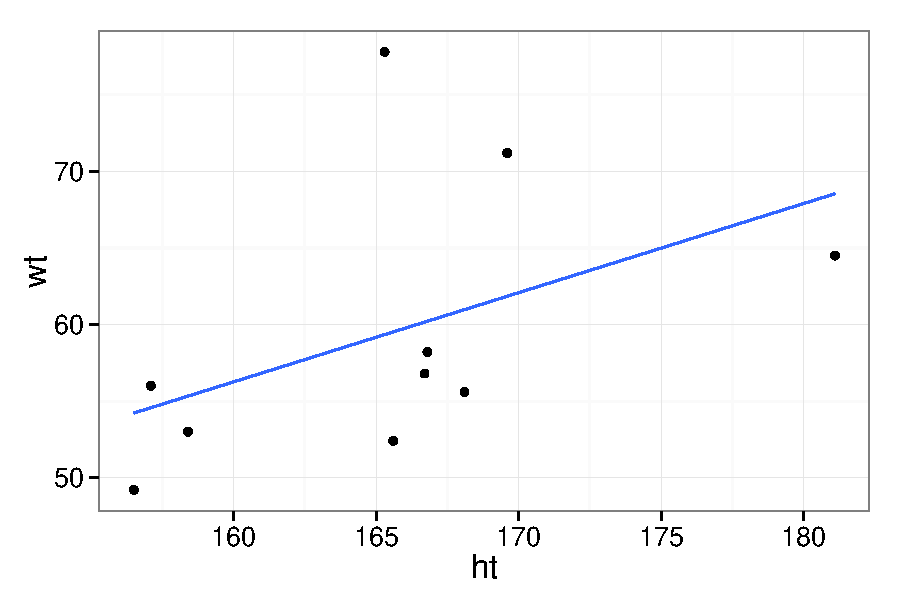
\includegraphics[width=.6\linewidth]{figure/p212} 

}



\end{knitrout}

\begin{problem}{2.1.3} Obtain the estimate of $\sigma^2$ and find the estimated standard errors of $\beta_{0}$ and $\beta_{1}$. Also find the estimated covariance between $\beta_{0}$ and $\beta_{1}$. Compute the t-tests for the hypotheses that $\beta_{0} = 0$ and that $\beta_{1} = 0$ and find the appropriate p-values using two-sided tests.
\end{problem}

$$\hat{\sigma ^ 2} = \frac{\sum_{i}{e_{i} ^ 2}}{n - 2} = 71.5017$$
$$\hat{Se}(\hat{\beta}_{1}) = \sqrt{\hat{\sigma ^ 2} \cdot \frac{1}{S_{XX}}} = 0.3892$$
$$\hat{Se}(\hat{\beta}_{0}) = \sqrt{\hat{\sigma ^ 2} \cdot (\frac{1}{n} + \frac{\bar{x} ^ 2}{S_{XX}})} = 64.4728$$
$$Cov(\hat{\beta}_{1}, \hat{\beta}_{0}) = -\hat{\sigma ^ 2} \frac{\bar{x}}{S_{XX}} = -25.07$$
$$t_{\beta_{0}} = \frac{\hat{\beta_{0}} - 0}{\hat{Se}(\hat{\beta}_{0})} = \frac{-36.8759}{64.4728} = -0.572$$
$$t_{\beta_{1}} = \frac{\hat{\beta_{1}} - 0}{\hat{Se}(\hat{\beta}_{1})} = \frac{0.5821}{0.3892} = 1.496$$
$$p_{\beta_{0}} = P(x > |t_{\beta_{0}}|; x \sim t(8)) = 0.583$$
$$p_{\beta_{1}} = P(x > |t_{\beta_{1}}|; x \sim t(8)) = 0.173$$
\\\\

\begin{problem}{2.10}
\textbf{Two-sample tests} One of the basic problems in elementary statistics is testing for equality of two means. If $\bar{y}_{j}, j = 0,1$, are the sample means, the sample sizes are $m_{j} , j = 0, 1$, and the sample standard deviations are $SD_{j}, j  =  0, 1$, then under the assumption that sample $j$ is $NID(\mu_{j}, \sigma^{2})$, the statistic 
$$t =\frac{\bar{y}_{1} - \bar{y}_{0}}{\hat{\sigma}\sqrt{1/m_{0} + 1/m_{1}} }$$
with $\hat{\sigma}^{2} = [( m_{0} - 1 ) SD_{0}^{2} + ( m_{1} - 1 ) SD_{1}^{2} ] / [ m_0 + m_1 - 2 ]$ is used to test $\mu_{0} = \mu_{1}$ against a general alternative. Under normality and the assumptions of equal variance in each population, the null distribution is $t \sim t(m_{0}+m_{1}-2)$.

For simplicity assume $m_{0} = m_{1} = m$, although the results do not depend on the equal sample sizes. Define a predictor $X$ with values $x_{i} = 0$ for $i = 1,\dots,m$ and $x_{i} = 1$ for $i = m+1,\dots,2m$. Combine the response $y_{i}$ into a vector of length $2m$, the first $m$ observations corresponding to population 0 and the remaining to population 1. In this problem we will fit the simple linear regression model for this $X$ and $Y$, and show that it is equivalent to the two-sample problem.
\end{problem}

\begin{problem}{2.10.1}
Show that $\bar{y} = ( \bar{y}_{0} + \bar{y}_{1} ) / 2$ , $\bar{x} = 1 / 2$ , $S_{XX}  =  m/2$, and $S_{XY} = m ( \bar{y}_1-\bar{y}_0 ) / 2$.
\end{problem}

$$\bar{y} = \frac{\sum_{i = 1}^{m}{y_{i}} + \sum_{i=m+1}^{2m}{y_{i}}}{2m} = \frac{\bar{y}_{0}m + \bar{y}_{1}m}{2m} = \frac{\bar{y}_{0} + \bar{y}_{1}}{2}$$
$$\bar{x} = \frac{\sum_{i = 1}^{m}{x_{i}} + \sum_{i=m+1}^{2m}{x_{i}}}{2m} = \frac{m}{2m} = \frac{1}{2}$$
$$S_{XX} = \sum_{i = 1}^{m}{(x_{i} - \frac{1}{2})^2} + \sum_{i=m+1}^{2m}{(x_{i} - \frac{1}{2})^2} = \frac{1}{4}\cdot 2m = \frac{m}{2}$$
$$S_{XY} = \sum_{i = 1}^{m}{(0 - \frac{1}{2})(y_{i} - \frac{\bar{y}_{0} + \bar{y}_{1}}{2})} + \sum_{i=m+1}^{2m}{(1 - \frac{1}{2})(y_{i} - \frac{\bar{y}_{0} + \bar{y}_{1}}{2})} = \frac{m}{2}(\bar{y}_{1} - \bar{y}_{0})$$

\begin{problem}{2.10.2}
Give the formulas for the OLS estimates of $\beta_{0}$ and $\beta_{1}$ in the simple linear regression model with the $Y$ and $X$ as specified in this problem. Interpret the estimates.
\end{problem}

$$\hat{\beta}_{1} = \frac{S_{XY}}{S_{XX}} = \frac{\frac{m}{2}(\bar{y}_{1} - \bar{y}_{0})}{\frac{m}{2}} = \bar{y}_{1} - \bar{y}_{0}$$
$$\hat{\beta}_{0} = \bar{y} - \bar{x}\hat{\beta}_{1} = \frac{\bar{y}_{0} + \bar{y}_{1}}{2} - \frac{1}{2}(\bar{y}_{1} - \bar{y}_{0}) = \bar{y}_{0}$$

$E(Y_{i}| X_{i} = 1) = \bar{y}_{1}$, $E(Y_{i}| X_{i} = 0) = \bar{y}_{0}$. Given $x = 1$, the estimated value of $y$ is equal to the mean value of population 1; given $x = 0$, the estimated value of $y$ is equal to the mean value of population 0;

\begin{problem}{2.10.3}
Find the fitted values and the residuals. Give an expression for RSS obtained by squaring and adding up the residuals and then dividing by the df.
\end{problem}

$$\hat{y}_{i} = \bar{y}_{0} + (\bar{y}_{1} - \bar{y}_{0})x_{i} = \Big\{ 
\begin{matrix}
  \bar{y}_{0} & x_{i} = 0  \\
  \bar{y}_{1} & x_{i} = 1 \\
 \end{matrix}$$
$$RSS = \sum_{i = 1}^{2m}{(y_{i} - \hat{y}_{i})} = \sum_{i = 1}^{m}{(y_{i} - \bar{y}_{0})^2} + \sum_{i = m+1}^{2m}{(y_{i} - \bar{y}_{1})^2} = (m - 1)SD_{0}^{2} + (m - 1)SD_{1}^{2}$$
$$\hat{\sigma^2} = \frac{RSS}{df} = \frac{(m - 1)SD_{0}^{2} + (m - 1)SD_{1}^{2}}{2m - 2} = \frac{SD_{0}^{2} + SD_{1}^{2}}{2}$$

\begin{problem}{2.10.4}
Show that the t-statistic for testing $\beta_{1} = 0$ is exactly the same as the usual two-sample t-test for comparing two groups with an assumption of equal within-group variance.
\end{problem}

$$\hat{Se}(\hat{\beta}_{1}) = \sqrt{\frac{1}{S_{XX}}\hat{\sigma^2}} = \sqrt{\frac{1}{m}(SD_{0}^{2} + SD_{1}^{2})}$$
$$t_{\beta_{1}} = \frac{\hat{\beta}_{1}}{\hat{Se}(\hat{\beta}_{1})} = \frac{\bar{y}_{1} - \bar{y}_{0}}{\sqrt{\frac{1}{m}(SD_{0}^{2} + SD_{1}^{2})}} \sim t(2m -2) = \frac{\bar{y}_{1} - \bar{y}_{0}}{\hat{\sigma}\sqrt{\frac{2}{m}}}$$
which is the same as the usual two-sample t-test for comparing two groups with an assumption of equal within-group variance.

\begin{problem}{2.10.5}
The group indicator is set to $x_{i} = 0$ for one group and $x_{i}  = 1$ for the other group. Suppose we used as the group indicator $x_{i}^{*} = -1$ for the first group and $x_{i}^{*} = +1$ for the second group. How will this change the estimates of $\beta_{0}$ and $\beta_{1}$ and the meaning of the test that $\beta_{1} = 0$? (Hint: Find values $a$ and $b$ such that $x_{i}^{*} = a(x_{i} + b)$ , and then apply Problem 2.9.1.)
\end{problem}

$$x_{i}^{*} = 2(x_{i} - 0.5) \rightarrow x_{i} = 0.5 \cdot x_{i}^{*} + 0.5$$
$$\beta_{1}^{*} = \beta_{1} \cdot 0.5$$
$$\beta_{0}^{*} = \beta_{0} + 0.5 \cdot \beta_{1}$$
$$\beta_{1}^{*} = 0 \iff \beta_{1} = 0$$

Since the response Y has not changed, the estimate of $\sigma^2$ will be unchanged. The test of the $\beta_{1}^{*}$ equal to 0 will be the same.

\begin{problem}{2.10.6}
(Data file: cathedral) The datafile contains the Height and Length in feet of 25 cathedrals, nine in the Romanesque style, and 16 in the later Gothic style. Consider only the first 18 rows of this data file, which contain all the Romanesque cathedrals and nine of the Gothic cathedrals, and consider testing the hypothesis that the mean length is the same for Romanesque and Gothic cathedrals against the alternative that they are different. Use these data to verify all the results of the preceding sections of this problem. (Hint: In the data file the group indicator Type is a text variable with values Romanesque and Gothic that you may need to convert to zeros and ones. In R, for example, the statement

> cathedral\$group <-
ifelse(cathedral\$Type==“Romanesque”, 0, 1)

will do it. Don’t forget to remove the last seven rows of the file, although if you do forget the test computed will still be a t-test of the hypothesis that the two types of cathedrals have the same mean height, but based on different data.)
\end{problem}

\textbf{Comparison between two-sample t-test (model\_1) and linear regression(model\_2)}

\begin{knitrout}
\definecolor{shadecolor}{rgb}{1, 1, 1}\color{fgcolor}\begin{kframe}
\begin{alltt}
\hlstd{data} \hlkwb{<-} \hlstd{cathedral}
\hlstd{data}\hlopt{$}\hlstd{group} \hlkwb{<-} \hlkwd{ifelse} \hlstd{(data}\hlopt{$}\hlstd{Type} \hlopt{==} \hlstr{"Romanesque"}\hlstd{,} \hlnum{0}\hlstd{,} \hlnum{1}\hlstd{)}
\hlstd{data} \hlkwb{<-} \hlstd{data[}\hlnum{1}\hlopt{:}\hlstd{(}\hlkwd{nrow}\hlstd{(data)}\hlopt{-}\hlnum{7}\hlstd{), ]}
\hlstd{model_1} \hlkwb{<-} \hlkwd{t.test} \hlstd{(Length} \hlopt{~} \hlstd{Type,} \hlkwc{data} \hlstd{= data,} \hlkwc{var.equal} \hlstd{=} \hlnum{TRUE}\hlstd{)}
\hlstd{model_2} \hlkwb{<-} \hlkwd{lm} \hlstd{(Length} \hlopt{~} \hlstd{group,} \hlkwc{data} \hlstd{= data)}
\hlstd{model_1}
\end{alltt}
\begin{verbatim}
## 
## 	Two Sample t-test
## 
## data:  Length by Type
## t = -1.634, df = 16, p-value = 0.1218
## alternative hypothesis: true difference in means is not equal to 0
## 95 percent confidence interval:
##  -153.43   19.87
## sample estimates:
##     mean in group Gothic mean in group Romanesque 
##                    408.7                    475.4
\end{verbatim}
\begin{alltt}
\hlkwd{summary} \hlstd{(model_2)}
\end{alltt}
\begin{verbatim}
## 
## Call:
## lm(formula = Length ~ group, data = data)
## 
## Residuals:
##    Min     1Q Median     3Q    Max 
## -183.7  -47.5   12.8   67.3  110.3 
## 
## Coefficients:
##             Estimate Std. Error t value Pr(>|t|)    
## (Intercept)    475.4       28.9   16.45  1.9e-11 ***
## group          -66.8       40.9   -1.63     0.12    
## ---
## Signif. codes:  0 '***' 0.001 '**' 0.01 '*' 0.05 '.' 0.1 ' ' 1
## 
## Residual standard error: 86.7 on 16 degrees of freedom
## Multiple R-squared:  0.143,	Adjusted R-squared:  0.0894 
## F-statistic: 2.67 on 1 and 16 DF,  p-value: 0.122
\end{verbatim}
\end{kframe}
\end{knitrout}

Note that the $t$ statistic and the P-value of this two models are the same.\\\\

\textbf{Comparison between linear regression (model\_2) and regression with scaled $X$ (model\_3)}

\begin{knitrout}
\definecolor{shadecolor}{rgb}{1, 1, 1}\color{fgcolor}\begin{kframe}
\begin{alltt}
\hlstd{data} \hlkwb{<-} \hlstd{cathedral}
\hlstd{data}\hlopt{$}\hlstd{group} \hlkwb{<-} \hlkwd{ifelse} \hlstd{(data}\hlopt{$}\hlstd{Type} \hlopt{==} \hlstr{"Romanesque"}\hlstd{,} \hlnum{0}\hlstd{,} \hlnum{1}\hlstd{)}
\hlstd{data} \hlkwb{<-} \hlstd{data[}\hlnum{1}\hlopt{:}\hlstd{(}\hlkwd{nrow}\hlstd{(data)}\hlopt{-}\hlnum{7}\hlstd{), ]}
\hlstd{data}\hlopt{$}\hlstd{group_1} \hlkwb{<-} \hlstd{(data}\hlopt{$}\hlstd{group} \hlopt{-} \hlnum{0.5}\hlstd{)} \hlopt{*} \hlnum{2}
\hlstd{model_3} \hlkwb{<-} \hlkwd{lm} \hlstd{(Length} \hlopt{~} \hlstd{group_1,} \hlkwc{data} \hlstd{= data)}
\hlkwd{summary}\hlstd{(model_3)}
\end{alltt}
\begin{verbatim}
## 
## Call:
## lm(formula = Length ~ group_1, data = data)
## 
## Residuals:
##    Min     1Q Median     3Q    Max 
## -183.7  -47.5   12.8   67.3  110.3 
## 
## Coefficients:
##             Estimate Std. Error t value Pr(>|t|)    
## (Intercept)    442.1       20.4   21.63  2.9e-13 ***
## group_1        -33.4       20.4   -1.63     0.12    
## ---
## Signif. codes:  0 '***' 0.001 '**' 0.01 '*' 0.05 '.' 0.1 ' ' 1
## 
## Residual standard error: 86.7 on 16 degrees of freedom
## Multiple R-squared:  0.143,	Adjusted R-squared:  0.0894 
## F-statistic: 2.67 on 1 and 16 DF,  p-value: 0.122
\end{verbatim}
\end{kframe}
\end{knitrout}

Note that the relationship between two $\beta_{1}$, $\beta_{0}$ is the same as what we prove in 2.10.5, and the $t$ statistic and the t-test remain the same. 
\\\\
\begin{problem}{2.13}
Heights of mothers and daughters (Data file: Heights)
\end{problem}

\begin{problem}{2.13.1}
Compute the regression of dheight on mheight, and report the estimates, their standard errors, the value of the coefficient of determination, and the estimate of variance. Write a sentence or two that summarizes the results of these computations.
\end{problem}

\begin{knitrout}
\definecolor{shadecolor}{rgb}{1, 1, 1}\color{fgcolor}\begin{kframe}
\begin{alltt}
\hlstd{data} \hlkwb{<-} \hlstd{Heights}
\hlstd{model} \hlkwb{<-} \hlkwd{lm}\hlstd{(dheight} \hlopt{~} \hlstd{mheight,} \hlkwc{data} \hlstd{= data)}
\hlkwd{summary}\hlstd{(model)}
\end{alltt}
\begin{verbatim}
## 
## Call:
## lm(formula = dheight ~ mheight, data = data)
## 
## Residuals:
##    Min     1Q Median     3Q    Max 
## -7.397 -1.529  0.036  1.492  9.053 
## 
## Coefficients:
##             Estimate Std. Error t value Pr(>|t|)    
## (Intercept)   29.917      1.623    18.4   <2e-16 ***
## mheight        0.542      0.026    20.9   <2e-16 ***
## ---
## Signif. codes:  0 '***' 0.001 '**' 0.01 '*' 0.05 '.' 0.1 ' ' 1
## 
## Residual standard error: 2.27 on 1373 degrees of freedom
## Multiple R-squared:  0.241,	Adjusted R-squared:  0.24 
## F-statistic:  435 on 1 and 1373 DF,  p-value: <2e-16
\end{verbatim}
\end{kframe}
\end{knitrout}

the OLS estimate of $\beta_{1}$ is 0.54175, the OLS estimate of $\beta_{0}$ is 29.91744, the standard error of the estimate of $\beta_{1}$ is 0.02596, the standard error of the estimate of $\beta_{0}$ is 1.62247. The coefficient of determination of this OLS model is $R^{2} = 0.2408$, the estimate of variance of the OLS model is $\hat{\sigma}^2 = 2.266 ^ 2 = 5.136$

The p-value of t-test is almost 0, suggesting that $\beta_{1} \neq 0$. $R^2 = 0.241$, so only about one-fourth of the variability in daughter’s height is explained by mother’s height.

\textbf{A 1 inch increase in mother's height will result in a 0.54 increase in daughter's height on average. (given all other predictors have the same value)}

\begin{problem}{2.13.2}
Obtain a 99\% confidence interval for $\beta_{1}$ from the data.
\end{problem}
\begin{comment} 
$\alpha = 0.01$, $t_{1-\alpha/2}(n-2) = 2.58$
$$\begin{aligned}
t_{\alpha/2}(n-2) &\leq& \frac{\hat{\beta}_{1} - \beta_{1}}{\hat{Se}(\hat{\beta}_{1})} &\leq& t_{1-\alpha/2}(n-2)\\
-2.58\cdot\hat{Se}(\hat{\beta}_{1}) &\leq& \hat{\beta}_{1} - \beta_{1} &\leq& 2.58\cdot\hat{Se}(\hat{\beta}_{1})\\
\hat{\beta}_{1} - 2.58\cdot\hat{Se}(\hat{\beta}_{1}) &\leq& \beta_{1} &\leq& \hat{\beta}_{1} + 2.58\cdot\hat{Se}(\hat{\beta}_{1})\\
0.475 &\leq& \beta_{1} &\leq& 0.609
\end{aligned}$$
\end{comment}
\begin{knitrout}
\definecolor{shadecolor}{rgb}{1, 1, 1}\color{fgcolor}\begin{kframe}
\begin{alltt}
\hlkwd{confint}\hlstd{(model,} \hlkwc{level}\hlstd{=}\hlnum{0.99}\hlstd{)}
\end{alltt}
\begin{verbatim}
##               0.5 %  99.5 %
## (Intercept) 25.7324 34.1025
## mheight      0.4748  0.6087
\end{verbatim}
\end{kframe}
\end{knitrout}

$\beta_{1} \in [0.475, ~0.609]$

\begin{problem}{2.13.3}
Obtain a prediction and 99\% prediction interval for a daughter
whose mother is 64 inches tall.
\end{problem}
\begin{knitrout}
\definecolor{shadecolor}{rgb}{1, 1, 1}\color{fgcolor}\begin{kframe}
\begin{alltt}
\hlkwd{predict}\hlstd{(model,} \hlkwd{data.frame}\hlstd{(}\hlkwc{mheight}\hlstd{=}\hlnum{64}\hlstd{),} \hlkwc{interval}\hlstd{=}\hlstr{"prediction"}\hlstd{,} \hlkwc{level}\hlstd{=}\hlnum{.99}\hlstd{)}
\end{alltt}
\begin{verbatim}
##     fit   lwr   upr
## 1 64.59 58.74 70.44
\end{verbatim}
\end{kframe}
\end{knitrout}

$y \in [58.740, ~70.438]$
\\\\
\begin{problem}{2.17}
Regression through the origin Occasionally, a mean function in which the intercept is known a priori to be 0 may be fit. This mean function is given by $$E(y|x) = \beta_{1}x$$
The residual sum of squares for this model, assuming the errors are independent with common variance $\sigma^{2}$ , is $RSS = \sum{(y_{i} - \beta x_{i})^2}$
\end{problem}

\begin{problem}{2.17.1}
Show that the least squares estimate of $\beta_{1}$ is $\hat{\beta}_{1} = \sum{x_{i}y_{i}} / \sum{x_{i}^{2}}$. Show that $\hat{\beta}_{1}$ is unbiased and that $Var(\hat{\beta}_{1}|X) = \sigma^{2} / \sum{x_{i}^2}$. Find an expression for $\sigma^{2}$. How many $df$ does it have?
\end{problem}

$$\hat{\beta}_{1} = \min_{\beta} \sum{(y_{i} - x_{i}\beta)^2} = \min_{\beta} f(\beta)$$
$$\frac{\partial f}{\partial \beta} = 0 \Rightarrow \sum{(y_{i} - x_{i}\beta)x_{i}} \Rightarrow \hat{\beta}_{1} = \frac{\sum{x_{i}y_{i}}}{\sum{x_{i}^{2}}}$$ 
$$E(\hat{\beta}_{1}) = E(\sum{\frac{x_{i}}{\sum{x_{i}^2}}\cdot y_{i}}) = \sum{\frac{x_{i}}{\sum{x_{i}^2}}\cdot x_{i}\beta} = \beta$$
$$Var(\hat{\beta}_{1}) = Var(\sum{\frac{x_{i}}{\sum{x_{i}^2}}\cdot y_{i}}) = \sum{\frac{x_{i}^2}{(\sum{x_{i}^2})^2}Var(y_{i})} = \frac{1}{\sum{x_{i}^2}}\sigma^2$$
$$\hat{\sigma^2} = \frac{\sum{(y_{i} - x_{i}\hat{\beta}_{1})^2}}{df}$$
$$df = n-1$$

\begin{problem}{2.17.2}
(Data file: snake) The data file gives $X$ = water content of snow on April 1 and $Y$ = water yield from April to July in inches in the Snake River watershed in Wyoming for $n = 17$ years from 1919 to 1935 (Wilm, 1950). Fit a regression through the origin and find $\hat{\beta}_{1}$ and $\hat{\sigma^2}$ . Obtain a 95\% confidence interval for $\beta_{1}$ . Test the hypothesis that the slope $\beta_{1} = 0.49$, against the alternative that $\beta_{1} > 0.49$.
\end{problem}

\begin{knitrout}
\definecolor{shadecolor}{rgb}{1, 1, 1}\color{fgcolor}\begin{kframe}
\begin{alltt}
\hlstd{data} \hlkwb{<-} \hlstd{snake}
\hlstd{model} \hlkwb{<-} \hlkwd{lm}\hlstd{(Y} \hlopt{~} \hlstd{X} \hlopt{-} \hlnum{1}\hlstd{,} \hlkwc{data} \hlstd{= data)}
\hlkwd{summary}\hlstd{(model)}
\end{alltt}
\begin{verbatim}
## 
## Call:
## lm(formula = Y ~ X - 1, data = data)
## 
## Residuals:
##    Min     1Q Median     3Q    Max 
## -2.421 -1.492 -0.194  1.651  3.077 
## 
## Coefficients:
##   Estimate Std. Error t value Pr(>|t|)    
## X   0.5204     0.0132    39.5   <2e-16 ***
## ---
## Signif. codes:  0 '***' 0.001 '**' 0.01 '*' 0.05 '.' 0.1 ' ' 1
## 
## Residual standard error: 1.7 on 16 degrees of freedom
## Multiple R-squared:  0.99,	Adjusted R-squared:  0.989 
## F-statistic: 1.56e+03 on 1 and 16 DF,  p-value: <2e-16
\end{verbatim}
\begin{alltt}
\hlkwd{confint}\hlstd{(model,} \hlkwc{level} \hlstd{=} \hlnum{0.95}\hlstd{)}
\end{alltt}
\begin{verbatim}
##    2.5 % 97.5 %
## X 0.4925 0.5483
\end{verbatim}
\end{kframe}
\end{knitrout}

\noindent $\hat{\beta}_{1} = 0.52039$, $\hat{\sigma^2} = 1.7 ^ 2 = 2.89$, $\beta_{1} \in [0.4925,~0.5483]$

\noindent Let $Z \sim t(16)$, then $P(Z > t) = P(Z > \frac{\hat{\beta}_{1} - 0.49}{\hat{Se}(\hat{\beta}_{1})}) = 0.017$

\begin{problem}{2.17.3}
Plot the residuals versus the fitted values, and comment on the
adequacy of the mean function with 0 intercept. In regression
through the origin, $\sum{\hat{e}_{i}} \neq 0$.
\end{problem}

\begin{knitrout}
\definecolor{shadecolor}{rgb}{1, 1, 1}\color{fgcolor}

{\centering 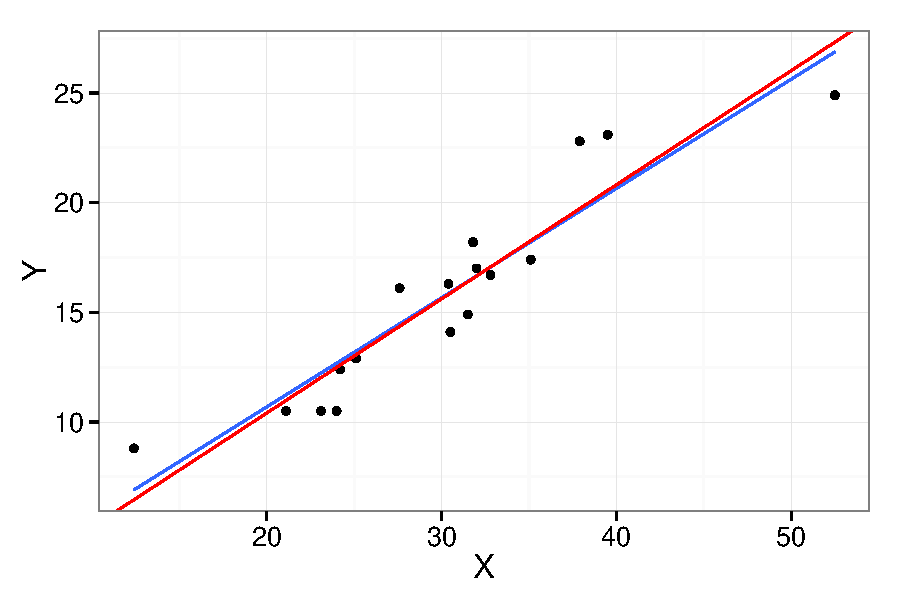
\includegraphics[width=.6\linewidth]{figure/p21731} 

}



\end{knitrout}

\noindent the Red line in this graph is the regression model fitted where intercept is known a priori to be 0, Blue line is the model fitted via standard OLS, Note that there exists little difference between this two line, which indicates that regression through origin point is OK in this problem.

\begin{knitrout}
\definecolor{shadecolor}{rgb}{1, 1, 1}\color{fgcolor}

{\centering 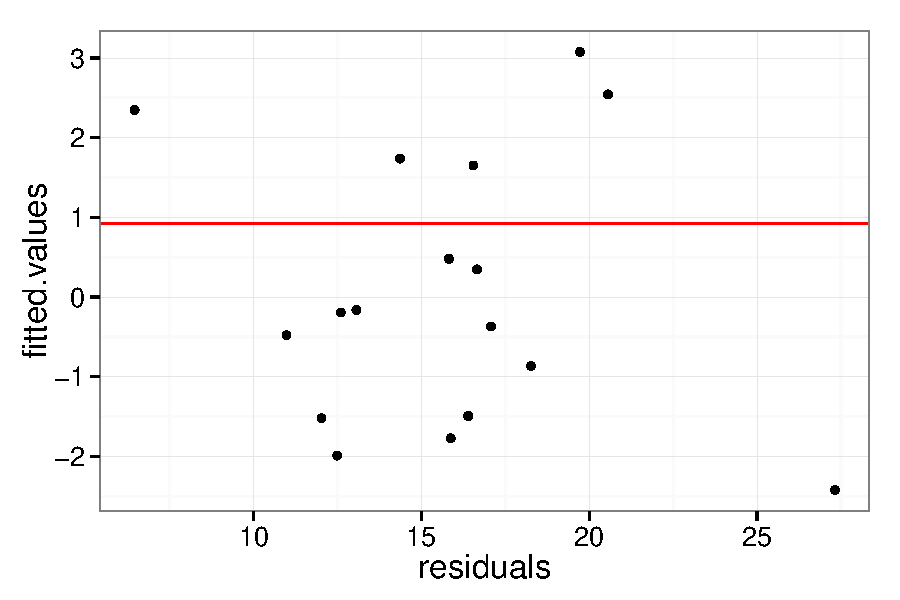
\includegraphics[width=.6\linewidth]{figure/p2173} 

}



\end{knitrout}

\noindent Red line in this graph illustrates the level of sum value of all residuals. Note that the Red line is far from $y = 0$, suggesting that $\sum{\hat{e}_{i}} \neq 0$.





\end{document}
